\chapter{Implementation}

As in the other projects, the camera calibration and object calculations will be implemented using Python and the OpenCV library that offers all necessary functionality to fulfill the task. \cite{pip_opencv} Additionally, the NumPy library is used for mathematical calculations. \cite{pip_numpy}

\section{Calibrating the videos}

To begin, the provided videos need to be used to calibrate the camera and obtain the intrinsic camera matrix. In general, the process that will be used has been described in the last project already \cite{report2}, therefore only a shorter summary will be provided. However, wherever changes in comparison to the last project were made, they will be mentioned.

According to the exercise description, for each video a separate intrinsic matrix should be calculated. \cite{cv_lecture_ex} This is done by first using the OpenCV function \texttt{findChessboardCorners()}, where the chessboard can be detected on each of the video frames. As a chessboard size to be detected by the function, 5x5 internal corners are used because this offered the best detection across the entire video in a short test. With bigger sizes, not enough frames were detected, especially in the parts of the video where the chessboard was moved to the edges of the image - where the important distortion information of the camera is visible.

Due to the large computational effort, not all frames where a chessboard has been detected can be used for the calibration however. Therefore, a selection of 40 frames for each video has been made. Like in the last project, 20 frames have been selected randomly using the Python function \texttt{random.sample()}. To further improve the detection results however, additionally 20 frames have been chosen manually, where the chessboard is held in the outer parts of the image - where the distortion of the camera is the strongest. This way, the camera calibration can work with more effective information available to undistort the edges of the image. In testing, this has slightly improved the undistortion, especially for video 1 in the top right corner.

Using the detected chessboard corners in the selected 40 frames and the OpenCV function \texttt{calibrateCamera()}, the intrinsic camera matrix of each video can be determined. Afterwards, each video frame can be undistorted with \texttt{undistort()} and then saved to the disk for further processing. In comparison to the original project, the intrinsic matrix has not been refined further this time, to keep the shape of the image identical. This is helpful for the next processing step.

To improve the undistortion results even more, unlike in the last project, the calibration is executed a second time, as recommended in the lecture. Therefore the once undistorted frames are taken and used as input for the identical calibration process again. Again, 20 random and the same 20 selected frames where the chessboard has been detected have been chosen for the calibration.

This has improved the undistortion noticeably, as can be seen in \autoref{fig:undist_2cal}. Especially in the corners, the parallel wall lines are less curved as before, so being better undistorted.

\begin{figure}[h]
    \centering
    \begin{subfigure}[b]{0.48\textwidth}
        \centering
        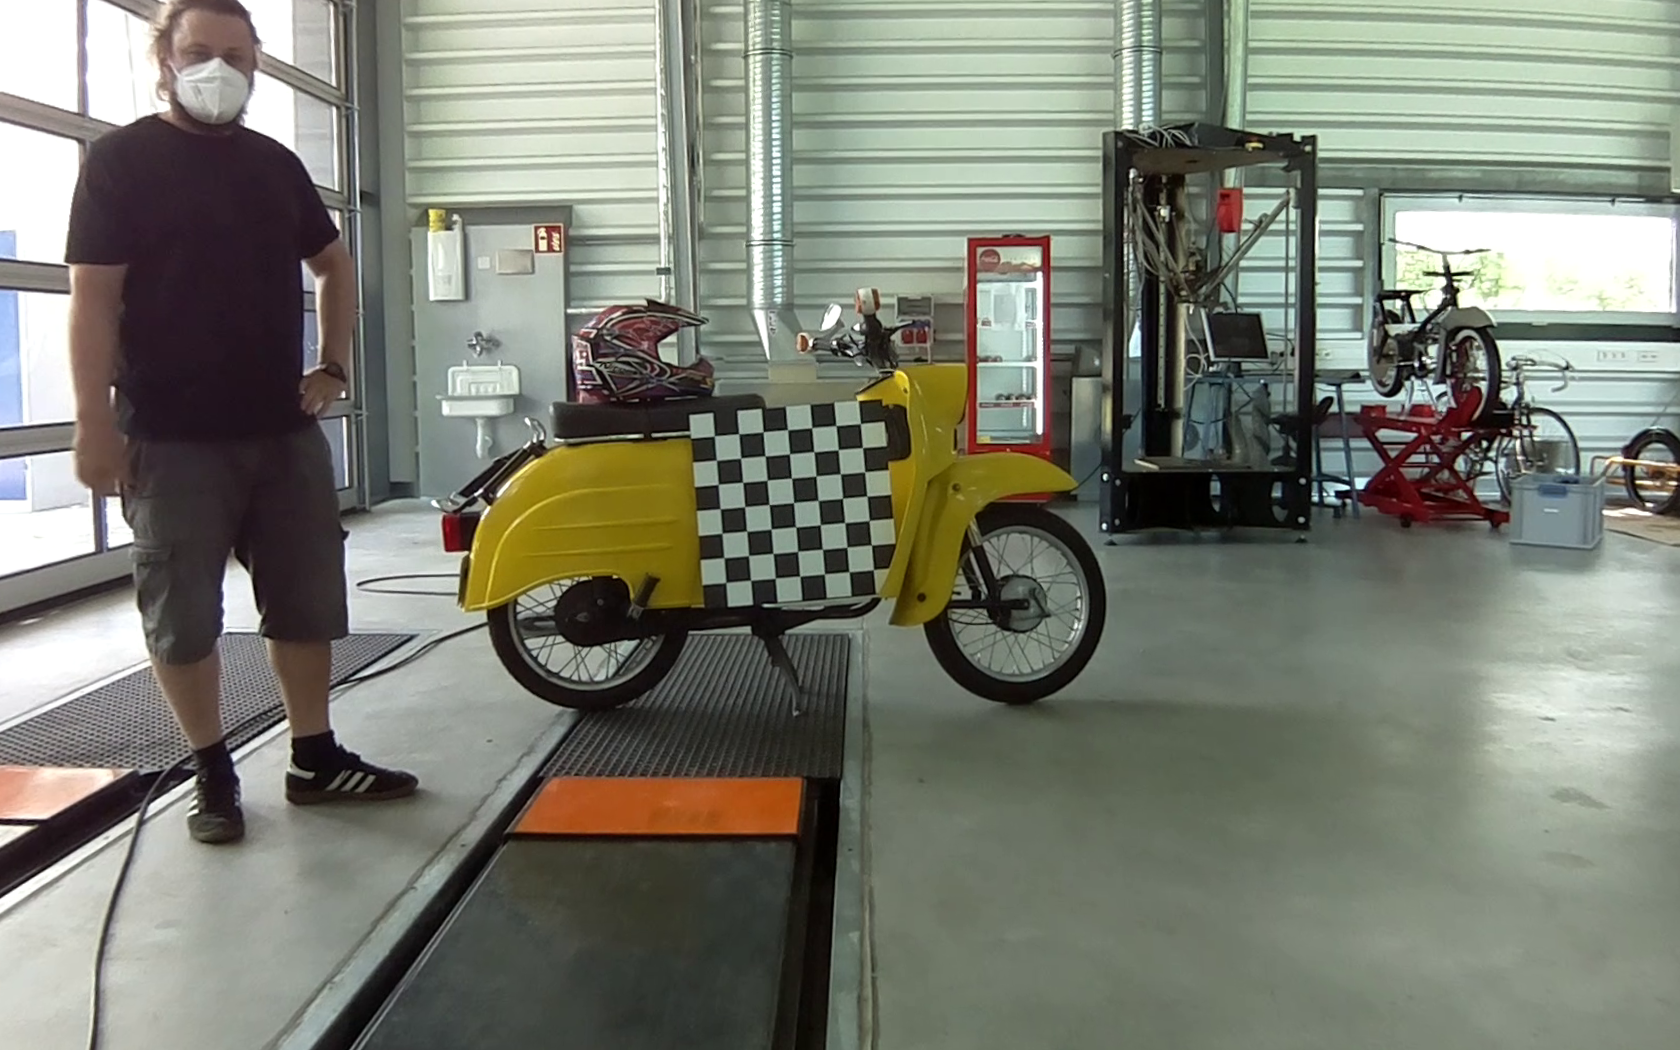
\includegraphics[width=\textwidth]{figures/video1_und1_20+20.png}
        \caption{After first calibration}
    \end{subfigure}
    \hfill
    \begin{subfigure}[b]{0.48\textwidth}
        \centering
        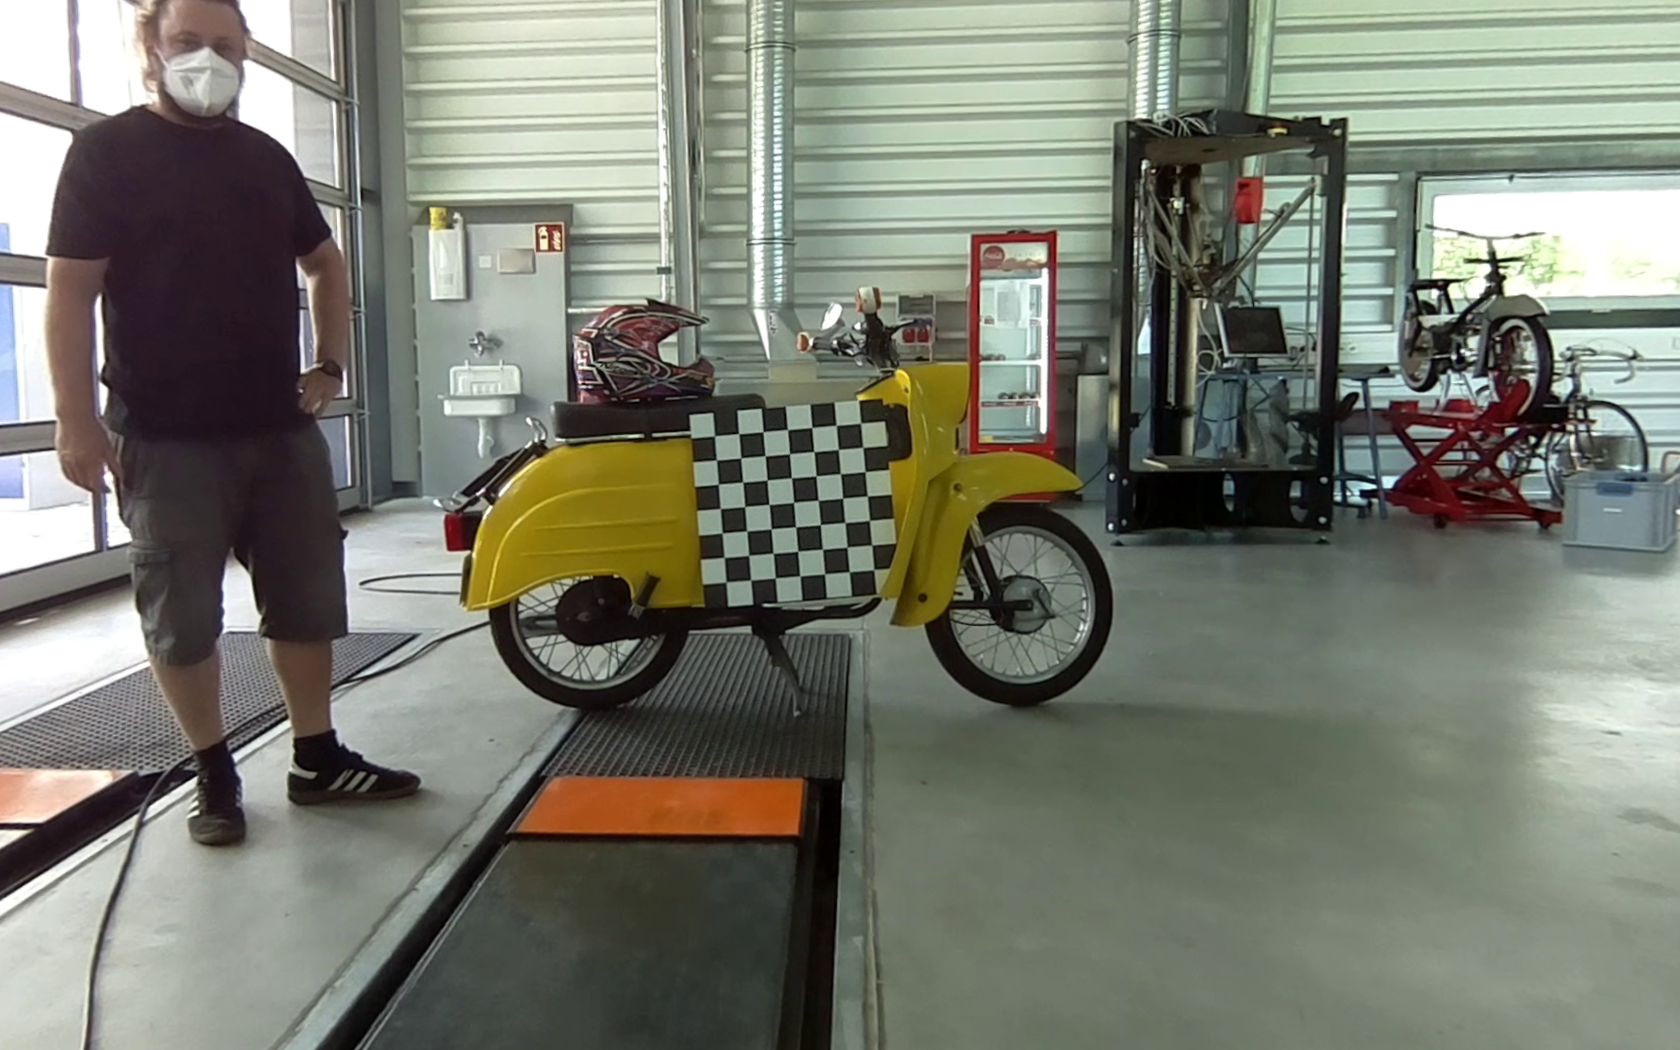
\includegraphics[width=\textwidth]{figures/video1_und2.png}
        \caption{After second calibration}
    \end{subfigure}
    \caption{Undistortion result of video 1 frame}
    \label{fig:undist_2cal}
\end{figure}

The amount of detected frames after the first and second calibration did not change significantly, as can be seen in \autoref{tbl:detectedframes}. Around 60 \% of all frames were detected in the videos.

\begin{table}[h]
    \centering
    \begin{tabular}{|l|l|l|l|l|}
        \hline
        \textbf{Video} & \textbf{Calibr.} & \textbf{Total frames}     & \textbf{Detected frames}                          & \textbf{Detection percentage}                    \\ \hline
        \textbf{0} & \textbf{I} & 671 & 411  & 61 \% \\ \hline
         & \textbf{II} &  & 430  & 64 \% \\ \hline
        \textbf{1} & \textbf{I} & 1056 & 637  & 60 \% \\ \hline
         & \textbf{II} &  & 572  & 54 \% \\ \hline
        \textbf{2} & \textbf{I} & 870 & 612  & 70 \% \\ \hline
         & \textbf{II} &  & 627  & 72 \% \\ \hline
        \end{tabular}
    \caption{Amount of detected frames with 5x5 chessboard in first and second calibration}
    \label{tbl:detectedframes}
\end{table}

The resulting intrinsic camera matrices were saved locally as files using the Python tool \texttt{pickle} (serialization) for further usage, so they could be loaded afterwards again. The intrinsic matrices for videos 0, 1 and 2 of the second calibration step can be seen in \autoref{eq:matrix0}, \autoref{eq:matrix1} and \autoref{eq:matrix2}. In theory, they should all be identical assuming the camera was not changed across the recordings. But there are differences up to 10 \% in the individual values of the matrices.

The main reason is that the images were undistorted before already, in the two-step process, with differing camera matrices per video. Therefore, the video frames were already undistorted by differing factors. Additionally, the camera may have been changed in between the recordings slightly. Moreover lighting conditions and other error sources could influence the result, which is always only an estimation.

\begin{equation} \label{eq:matrix0}
    M_0 =
    \begin{pmatrix}
        1285.1265 & 0 & 801.0578\\
        0 & 1284.44665 & 445.72247\\
        0 & 0 & 1
    \end{pmatrix}
\end{equation}

\begin{equation} \label{eq:matrix1}
    M_1 =
    \begin{pmatrix}
        1160.63588 & 0 & 780.77692\\
        0 & 1161.66796 & 477.22944\\
        0 & 0 & 1
    \end{pmatrix}
\end{equation}


\begin{equation} \label{eq:matrix2}
    M_2 =
    \begin{pmatrix}
        1304.50899 & 0 & 763.9381\\
        0 & 1303.83037 & 474.96704\\
        0 & 0 & 1
    \end{pmatrix}
\end{equation}

\section{Determining object dimensions}

Next, the task is to determine the size of the 3D printer. It is known the chessboard has the size 50 x 50 cm and is positioned perpendicular to the camera and 3D printer. The chessboard is in the same plane as the 3D printer. Also, an undistorted frame of the video is available where pixel values of the objects can be read from, as can be seen with the red and green lines in \autoref{fig:chessboard_width}.

\begin{figure}[h]
    \centering
    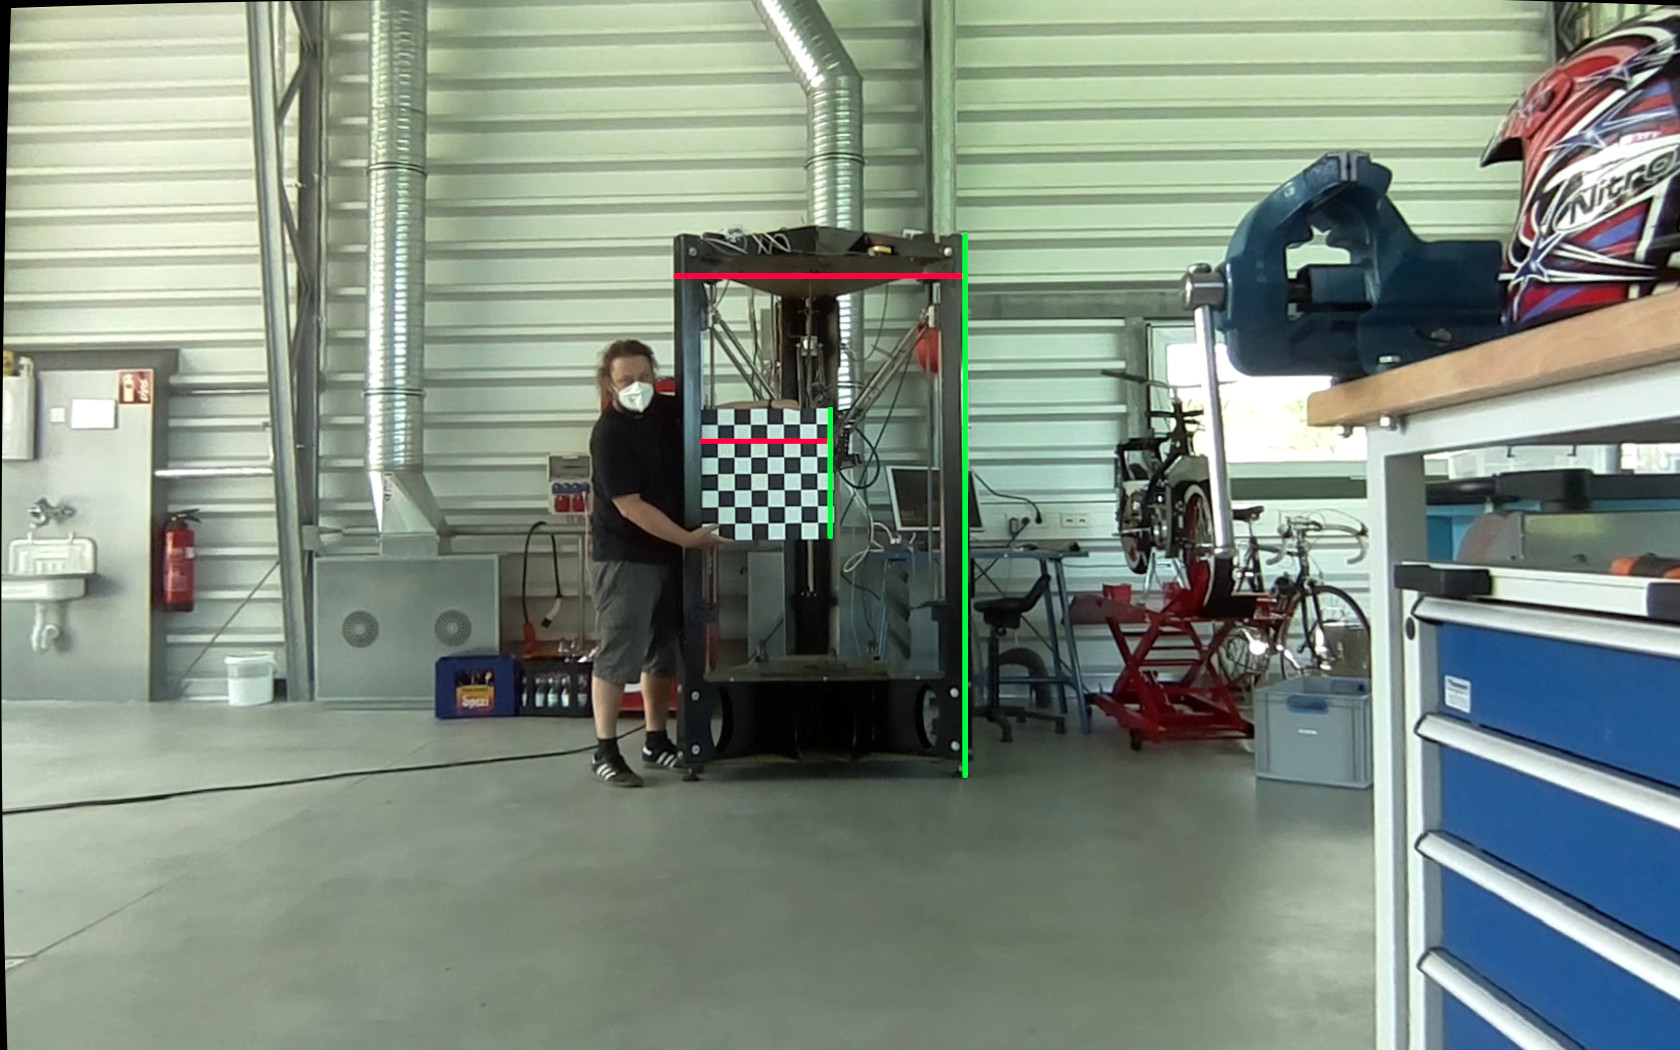
\includegraphics[width=0.6\textwidth]{figures/vid2_sizecalc.jpg}
    \caption{Dimensions of objects in video 2}
    \label{fig:chessboard_width}
\end{figure}

Using this information, it is possible to calculate the width and height of the printer. First, the pixel values of the chessboard $C$ and printer $P$ width and height need to be read off the image. The determined values can be seen in \autoref{eq:widths} (width) and \autoref{eq:heights} (height), based on the last frame of the undistorted video 2.

\begin{equation} \label{eq:widths}
    C_{px}^w = 833 - 700 px = 133 px \quad
    P_{px}^w = 968 - 674 px = 294 px
\end{equation}

\begin{equation} \label{eq:heights}
    C_{px}^h = 539 - 406 px = 133 px \quad
    P_{px}^h = 778 - 233 px = 545 px
\end{equation}

Using these values, it is now possible to set up a ratio between pixels and \enquote*{real-world} values in cm, as can be seen in \autoref{eq:sizecalculation}.

\begin{equation} \label{eq:sizecalculation}
    \frac{C_{cm}}{C_{px}} = \frac{P_{cm}}{P_{px}}
\end{equation}

All values except for $P_{cm}$ are available, which is why the equation can be solved for it, as seen in \autoref{eq:sizecalculationch}, resulting in the real-world size of the printer.

\begin{equation} \label{eq:sizecalculationch}
    \begin{split}
        P_{cm} & = \frac{C_{cm} * P_{px}}{C_{px}}\\
        P_{cm}^w & = \frac{50 cm * 294 px}{133 px} = 110 cm\\
        P_{cm}^h & = \frac{50 cm * 545 px}{133 px} = 205 cm
    \end{split}
\end{equation}

The estimation yields that the 3D printer is 110 cm wide and 205 cm high.

\section{Determining object distances}

Now, the distances of the 3D printer and the Schwalbe need to be determined. Using video 0, the approach can be evaluated first because the distance to the chessboard is already known to be 250 cm. Therefore the upcoming calculations should yield a similar result for video 0.

As stated in the project notes \cite{cv_lecture_ex}, it is possible to assign every point $\vec{z}$ in the two-dimensional image plane a line $L$ that maps them to a line in the three-dimensional room using the intrinsic camera matrix $K$, as seen in \autoref{eq:line}.

\begin{equation} \label{eq:line}
    L = \left\{ \begin{pmatrix} \lambda_1 \\ \lambda_2 \\ \lambda_3 \end{pmatrix} = d K^{-1} \begin{pmatrix} z_1 \\ z_2 \\ 1 \end{pmatrix} \middle\vert \; d \in \mathbb{R}; \begin{pmatrix} \lambda_1 \\ \lambda_2 \\ \lambda_3 \end{pmatrix} \in \mathbb{R}^3 \right\}
\end{equation}

The lines \enquote{begin} (or more exact, intersect) in the origin of the world coordinate system, which is in this case the camera itself. This determination is sufficient since only the relative distances to the camera are needed, and not the actual placement in the room or any other relative system. To better visualize the problem, in \autoref{fig:ovviz}, the situation of the camera, the image plane and the object plane in the room is visualized in a top-down view.

\begin{figure}[h]
    \centering
    \includegraphics[width=0.9\textwidth]{figures/CV_drawing}
    \caption{Top-down view on the camera and chessboard in the room}
    \label{fig:ovviz}
\end{figure}

On the left, the camera sends out the line rays capturing the borders of the chessboard. The image plane $w_p$ shows the 2D image of the chessboard, where the upper point crossing the line $L_l$ is the left side of the chessboard, while the lower point is the right side of the chessboard. The actual chessboard in the three-dimensional room is in further distance and marked with $w_m$. Both planes are perpendicular to the camera.

The values $w_p$ (width of chessboard in pixels), $w_m$ (width of chessboard in [centi]meters) and the lines $L_l$ and $L_r$ are known. Unknown are the values $d_p$ (distance between camera and image plane in pixels) and $d_m$ (distance between camera and object plane in [centi]meters). $d_m$ is exactly the distance to the chessboard that needs to be found.

Since the real chessboard is placed perpendicular to the camera, it is possible to find two similar triangles in the image - one smaller one between camera and image plane, and one bigger one between camera and the actual object plane. This is simplified in \autoref{fig:ovvizs} with the green and the red triangles.

\begin{figure}[h]
    \centering
    \includegraphics[width=0.8\textwidth]{figures/CV_drawing2}
    \caption{Simplified view of similar triangles}
    \label{fig:ovvizs}
\end{figure}

In similar triangles, the ratio between the two adjacent/opposite sides of the triangles is constant. Using this idea, it is possible to define a ratio between the two triangles as in \autoref{eq:similars}.

\begin{equation} \label{eq:similars}
    \frac{w_p / 2}{d_p} = \frac{w_m / 2}{d_m}
\end{equation}

As seen in the images, $d_m$ is the actual distance between camera and the chessboard in the \enquote{real-world} unit (here centimeters due to $w_m = 50 cm$). Therefore, \autoref{eq:similars} can now be solved for the sought $d_m$, like in \autoref{eq:distcalc}.

\begin{equation} \label{eq:distcalc}
    d_m = \frac{w_m * d_p}{w_p}
\end{equation}

To be able to calculate $d_m$, the only missing value is $d_p$. All other values are known to this point. However, this missing value can be determined using trigonometry if the angle $\alpha$ would be known (seen in \autoref{fig:ovviz}). But the angle between the lines is also not an unknown value, since it can be calculated as the angle between the two lines $L_l$ and $L_r$ at the intersection point. This can be done using the dot product of two vectors, here the direction vectors of the lines $L_l$ and $L_r$. The formula can be seen in \autoref{eq:alphacalc}. \cite{dotproduct}

\begin{equation} \label{eq:alphacalc}
    \alpha = \arccos{ \left(
        \frac{ L_l \centerdot L_r}{\lVert L_l \rVert \lVert L_r \rVert}  
        \right)}
\end{equation}

Using the calculated angle, with the trigonometric function $\tan$ the distance $d_p$ can be calculated, as seen in \autoref{eq:distcalcpx}. \cite{trigo}

\begin{equation} \label{eq:distcalcpx}
    d_p = \frac{w_p / 2}{\tan{\left(\alpha/2\right)}} = \frac{w_p}{2 \tan{\left(\alpha/2\right)}}
\end{equation}

\autoref{eq:similars} and \autoref{eq:distcalcpx} can now be put together and simplified, to be able to calculate the actual distance $d_m$ like in \autoref{eq:summarize}.

\begin{equation} \label{eq:summarize}
    d_m = \frac{w_m}{2\tan{\left(\alpha/2\right)}}
\end{equation}

With this formula, it is possible to calculate the distance estimation for each video using its intrinsic camera matrix, two image points $\vec{z_1}$ and $\vec{z_2}$ of chessboard and the real-world width of the chessboard $w_m = 50 cm$. The upcoming calculations have been made using the NumPy library for Python.

\subsection*{Video 0 (Reference)}

\begin{equation} \label{eq:video0}
    \begin{aligned}[t]
        \vec{z_1} &= \begin{pmatrix} 668 & 499 & 1 \end{pmatrix}^T \\
        \vec{z_2} &= \begin{pmatrix} 912 & 499 & 1 \end{pmatrix}^T
    \end{aligned}
    \qquad 
    \begin{aligned}[t]
        \alpha &= 0.1891218436272016\\
        d_m &= 263.59 cm
    \end{aligned}
\end{equation}

The error compared to the expected distance value of $250 cm$ is $\approx5 \%$.

\subsection*{Video 1 (Schwalbe)}

\begin{equation} \label{eq:video1}
    \begin{aligned}[t]
        \vec{z_1} &= \begin{pmatrix} 691 & 439 & 1 \end{pmatrix}^T \\
        \vec{z_2} &= \begin{pmatrix} 886 & 420 & 1 \end{pmatrix}^T
    \end{aligned}
    \qquad 
    \begin{aligned}[t]
        \alpha &= 0.16825217564450048\\
        d_m &= 296.47 cm
    \end{aligned}
\end{equation}

\subsection*{Video 2 (3D Printer)}

\begin{equation} \label{eq:video2}
    \begin{aligned}[t]
        \vec{z_1} &= \begin{pmatrix} 700 & 410 & 1 \end{pmatrix}^T \\
        \vec{z_2} &= \begin{pmatrix} 833 & 410 & 1 \end{pmatrix}^T
    \end{aligned}
    \qquad 
    \begin{aligned}[t]
        \alpha &= 0.10173949799169739\\
        d_m &= 491.03 cm
    \end{aligned}
\end{equation}

As the intrinsic matrixes have been calculated for each video only, they should not be interchangeable between the videos. Regardless, out of curiosity, the matrices of video 1 and 2 have also been used for the estimation of the distance in video 0. For matrix 1, this has yielded a value of $237.89cm$ (error $\approx5 \%$), while for matrix 2 the value $267.47cm$ (error $\approx7 \%$) has been determined.

As the error for all values is relatively similar, it can be expected the matrices for the other videos also seem to be accurate enough for video 1 amd video 2. But without knowing the actual distances in video 1 and 2, it is not possible to evaluate these results further.
